% ****** Start of file apssamp.tex ******
%
%   This file is part of the APS files in the REVTeX 4.2 distribution.
%   Version 4.2a of REVTeX, December 2014
%
%   Copyright (c) 2014 The American Physical Society.
%
%   See the REVTeX 4 README file for restrictions and more information.
%
% TeX'ing this file requires that you have AMS-LaTeX 2.0 installed
% as well as the rest of the prerequisites for REVTeX 4.2
%
% See the REVTeX 4 README file
% It also requires running BibTeX. The commands are as follows:
%
%  1)  latex apssamp.tex
%  2)  bibtex apssamp
%  3)  latex apssamp.tex
%  4)  latex apssamp.tex
%
\documentclass[%
 reprint,
%superscriptaddress,
%groupedaddress,
%unsortedaddress,
%runinaddress,
%frontmatterverbose, 
%preprint,
%preprintnumbers,
%nofootinbib,
%nobibnotes,
%bibnotes,
 amsmath,amssymb,
 aps,
%pra,
%prb,
%rmp,
%prstab,
%prstper,
%floatfix,
]{revtex4-2}

\usepackage{graphicx}% Include figure files
\usepackage{dcolumn}% Align table columns on decimal point
\usepackage{bm}% bold math
\usepackage{url}
\usepackage{algorithm}
\usepackage{algpseudocode}
%\usepackage{hyperref}% add hypertext capabilities
%\usepackage[mathlines]{lineno}% Enable numbering of text and display math
%\linenumbers\relax % Commence numbering lines

%\usepackage[showframe,%Uncomment any one of the following lines to test 
%%scale=0.7, marginratio={1:1, 2:3}, ignoreall,% default settings
%%text={7in,10in},centering,
%%margin=1.5in,
%%total={6.5in,8.75in}, top=1.2in, left=0.9in, includefoot,
%%height=10in,a5paper,hmargin={3cm,0.8in},
%]{geometry}

\begin{document}

\preprint{APS/123-QED}

\title{Constructing a Maximum Tension Coordinate in Cosmology with Neural Networks}
% \thanks{A footnote to the article title}%

\author{Yi Jer Loh}
 \email{yjl34@cam.ac.uk}
\author{Will Handley}
 \email{wh260@cam.ac.uk}
\affiliation{%
 Cavendish Laboratory, 19 J.J. Thomson Avenue, Cambridge CB3 0HE, UK
}%

\date{\today}

\begin{abstract}
Tensions in cosmology, such as the Hubble tension and the $\Omega_m$ - $\sigma_8$ tension, are rising as measurement precision improves over recent years. We develop on the idea of finding the maximum tension possible between two cosmological datasets. We use a simple neural network with a single hidden layer to learn a function of the parameter space which maximises the tension between the two datasets. This function is a mapping from a high-dimensional parameter space to a 1D coordinate, which we call the \textit{tension coordinate}. We apply this method to the \textit{Planck} and DES datasets on the following parameters: physical baryon density $\Omega_b h^2$, matter density $\Omega_m$, Hubble constant $H_0$, optical depth to reionisation $\tau$, matter fluctuation amplitude $\sigma_8$, and scalar power law index $n_s$. We first use all six parameters on our neural network, and obtain a marginalised Bayes factor of $\log R_t = -16.8 \pm 0.5$, which is significantly more tension that if we assumed that the distributions were Gaussian. We then apply our neural network to pairs of parameters to identify the parameters which contain the most tension. Our two methods are able to identify $H_0$, $\Omega_m$ and $\Omega_b h^2$ as the parameters which contribute most to the tension.
\end{abstract}

%\keywords{Suggested keywords}%Use showkeys class option if keyword
                              %display desired
\maketitle

%\tableofcontents


\section{Introduction} \label{intro}

With cosmological measurements becoming more precise over recent years, disagreements between different datasets and methods have begun to emerge. Observations of parameters surrounding the cosmological constant cold dark matter ($\Lambda \textrm{CDM}$) model have yielded discrepancies, more commonly referred to as \textit{tensions}, of close to $5\sigma$ -- the gold standard of significance in particle physics \cite{Franklin2013}. 

One such tension is the \textit{Hubble tension}. The debate over the Hubble constant's value is one that is hardly new, but in recent years has risen to prominence in cosmology. Disagreement over the Hubble constant began between de Vaucouleurs and Sandage in the 1980s \cite{deVaucouleurs1986, Sandage1975}, and it has now developed into an area of contention between early- and late-universe cosmologists \cite{Planck2020, Abbott2018, Freedman2020, Riess2019, Wong2019}. As it stands, measurements by these two factions are at significant tension of around $5\sigma$ at the most extreme, as shown in Figure \ref{H0_tension}. This has earned the Hubble tension an apt label of a cosmological \textit{crisis}.


\begin{figure}
    \includegraphics[width=0.8\columnwidth]{../plots/H0 tension.png}
    \centering
    \caption{A compilation of recent measurements of the Hubble constant $H_0$. The top two measurements are from early-universe datasets using $\Lambda$CDM cosmology \cite{Planck2020, Abbott2018}, while the remaining three are from late-universe datasets based off local distance ladder measurements \cite{Freedman2020, Riess2019, Wong2019}. The tension between the \textit{Planck} and SH0ES measurements currently stands at $4.7 \sigma$.}
    \label{H0_tension}
\end{figure}


In addition to the Hubble constant, less severe tensions also exist. Discrepancies of $3\sigma$ have been reported with respect to the matter density $\Omega_m$ and rate of growth of structure $\sigma_8$, between the Cosmic Microwave Background (CMB) data collected by \textit{Planck} and the weak lensing-based Kilo Degree Survey (KiDS) \cite{Heymans2021}. This tension also exist between the \textit{Planck} and the weak lensing-based Dark Energy Survey (DES), which we explore in this paper. Similarly, there has been arguments made for the existence of a ``curvature tension", with inconsistencies of $2.5 \sigma$ to $3 \sigma$ between CMB data alluding to a closed curved universe and the tenet of flat curvature in $\Lambda$CDM cosmology \cite{Handley2021Closed}.

These tensions raise questions surrounding the validity of the well-established, well-tested standard cosmological model -- the $\Lambda$CDM. Are these tensions just an artefact of systematic errors from collecting and analysing datasets? Or do these tensions hint at something more fundamental -- perhaps a modification to the standard model, or more excitingly new physics to take the place of the old one?

However, before we make that leap into the realm of new physics, it is essential for us to examine how tension is quantified. With cosmological datasets being multi-dimensional, the problem of quantifying discrepancies is non-trivial. Datasets that appear to be in mild tension, such as the Dark Energy Survey (DES) Y1 and Planck datasets, have been reported to be consistent when using the canonical Bayes factor $R$ \cite{Handley2019}. This is troubling, and is a reflection of the difficulty of the problem. With tensions likely to increase as measurement precision increases, a variety of tension metrics have been proposed in recent literature \cite{Charnock2017} to better understand the problem at hand.

This paper aims to develop the idea of coordinates of maximum tension. With cosmological datasets, larger tensions often exist across multiple parameters rather than within each parameter on its own. A good example would be the $3 \sigma$ tension between $\Omega_m$ and $\sigma_8$ -- the tension is obvious in a two-dimensional plot between these two parameters, but is not as significant when the parameters are inspected individually, as illustrated in Figure \ref{omegam_sigma8}. In a high-dimensional parameter space, it is thus likely that there exists a hidden combination of parameters which exacerbates and maximises tension.

\begin{figure}
    \includegraphics[width=0.9\columnwidth]{../plots/omegam_sigma8.png}
    \centering
    \caption{The main plot shows a two-dimensional marginalised distribution of the \textit{Planck} and DES datasets in the $\Omega_m$ - $\sigma_8$ plane, where the solid contours contain 68\% and 95\% of the marginalised probability mass. The two smaller plots are the one-dimensional marginalised distributions of both datasets in each   parameter.}
    \label{omegam_sigma8}
\end{figure}

In this paper, we explore a non-linear function of parameters for which the marginalised tension is maximised. A neural network is used to achieve this mapping, since the non-Gaussian nature of certain cosmological parameters renders an analytical approach challenging. This tension coordinate is then applied to the \textit{Planck} and DES Y1 datasets. Such an approach could allow us to develop a better intuition of the source of tension, and verify the large tensions that currently exist in $H_0$ and the $\Omega_m$-- $\sigma_8$ plane.



\section{Background}

\subsection{Bayesian Statistics}

We use the following notation of Bayesian statistics, with Bayes' theorem written as
\begin{equation}
    P(\theta|D) = \frac{P(D|\theta)P(\theta)}{P(D)} \, \longrightarrow \, \mathcal{P}_D(\theta) = \frac{\mathcal{L}_D(\theta) \pi(\theta)}{\mathcal{Z}_D}.
\end{equation}
The posterior is denoted as $\mathcal{P}_D$, likelihood as $\mathcal{L}_D$, prior as $\pi$, and evidence as $\mathcal{Z}_D$. Note that the subscript here represents the dataset-dependence of these distributions. 

The Bayesian evidence $\mathcal{Z}_D$ is defined as 
\begin{equation}
    \mathcal{Z}_D = \int \mathcal{L}_D \pi \ \rm{d} \theta.
\end{equation}
Also known as the marginal likelihood in statistical literature \cite{Trotta2008}, the evidence is often deemed to be a natural value for model and dataset comparisons within the Bayesian framework. However, the calculation of the evidence was historically computationally prohibitive, as it involves a multi-dimensional integral over the entire parameter space. Fortunately, there are now several tried-and-tested numerical methods that can reliably estimate the evidence, including thermodynamic integration \cite{Lartillot2006} and nested sampling \cite{Skilling2006, Handley2015}.


\subsection{Bayes Factor $R$}

The canonical Bayes factor $R$ \cite{Marshall2006} is our tension metric of choice, and forms the basis of our method in this paper. With two datasets $A$ and $B$, the Bayes factor is expressed as
\begin{equation}
    R = \frac{\mathcal{Z}_{AB}}{\mathcal{Z}_A \mathcal{Z}_B}, \quad \rm{with} \ \mathcal{Z}_{AB} = \int \mathcal{L}_A \mathcal{L}_B \pi \ \rm{d}\theta.
\end{equation}
This factor is defined as the ratio between the probability of $A$ and $B$ describing the same parameter space and the probability of $A$ and $B$ describing separate parameter spaces. A value of $R \gg 1$ indicates datasets that are in agreement, and $R \ll 1$ indicates discrepant datasets.

The Bayes factor can be re-expressed as 
\begin{equation}
    R = \int \frac{\mathcal{P}_A \mathcal{P}_B}{\pi} \ \rm{d}\theta.
\end{equation}
This is a more convenient expression to work with, since it sidesteps the numerical complexity of computing evidences. This form of the Bayes factor also makes explicit its prior-dependence, which is arguably a concern \cite{Handley2019}. A broader prior would increase the factor $R$, whilst a narrower prior would reduce $R$ and thus increase tension. Such a dependence means that $R$ is able to hide potential discrepancies with a broad prior. On the other hand, consistent datasets with sensible priors \textit{cannot} be reported to be in tension by the Bayes factor. This means that a value of $R$ indicating tension does in fact point to disagreeing datasets, hence low values of $R$ must be taken more seriously than higher values of $R$.


\subsection{Tension Coordinate}

Many tension quantification methods, including the Bayes factor, have the desirable characteristic of being independent of the choice of parameters and the direction in the parameter space. However, it would also be interesting to be able to describe the spatial structure of the tension, i.e. which parameters contribute most to the tension. As alluded to in the introduction of this paper, it is very probable that there exists a combination of parameters, or more generally a function of the parameter space, which maximises tension between two datasets. The output of such a function is what we call the \textit{tension coordinate}. 

% This coordinate can be expressed as $t = T(\theta)$, where $\theta$ represents the parameter space.

% This idea could be a first step in better understanding the sources of tension between datasets, particularly when one believes there to be more tension than one would expect from a global tension metric.

In this paper, tension is quantified using the Bayes factor $R$. We minimise $R$, calculated in the tension coordinate, to achieve maximum tension. We first demonstrate the tension coordinate for the ideal case of two Gaussian distributions representing two separate datasets. Then, we approach the tension coordinate more practically to tackle non-Gaussian distributions.

\subsubsection{Gaussian example} \label{gaussian_tension}

Let there be two datasets $A$ and $B$ represented by two Gaussian distributions with shared parameters $\theta$. $A$ and $B$ have mean vectors of $\mu_A$ and $\mu_B$, and covariance matrices of $\Sigma_A$ and $\Sigma_B$, respectively. The natural log of the Bayes factor $R$ between these two distributions is written as \cite{Handley2019}
\begin{align}
    \log R &= - \frac{1}{2} (\mu_A - \mu_B)^T (\Sigma_A + \Sigma_B)^{-1} (\mu_A - \mu_B) \\
    &= - \frac{1}{2} \mu^T \Sigma^{-1} \mu
\end{align}
where $\mu = \mu_A - \mu_B$ and $\Sigma = \Sigma_A + \Sigma_B$.

Define the one-dimensional tension coordinate as a linear combination of the parameters, $t = n^T \theta$. The vector $n$ can be naturally described as the direction of maximum tension. To map the Gaussian distributions onto $t$, we marginalise the distributions onto the hyperplanes perpendicular to $n$. This gives a marginalised Bayes factor of
\begin{align}
    \log R_t &= -\frac{1}{2} \big( n^T \mu \big)^T \big( n^T \Sigma n \big)^{-1} \big( n^T \mu \big) \\
    &= -\frac{\big( n^T \mu \big)^2}{2 n^T \Sigma n}.
\end{align}

Minimising $\log R_t$ with respect to $n$, which maximises the marginalised tension, gives the direction of maximum tension as
\begin{equation}
    n \propto \Sigma^{-1} \mu = (\Sigma_A + \Sigma_B)^{-1} (\mu_A - \mu_B).
\end{equation}
Substituting this back into the tension coordinate returns
\begin{equation}
    t = n^T \theta \propto (\mu_A - \mu_B)^T (\Sigma_A + \Sigma_B)^{-1} \theta
\end{equation}
where $t$ is defined up to a normalisation constant.

\subsubsection{Non-Gaussian case} \label{non_gaussian}

Datasets with non-Gaussian distributions bring more complexity to the tension coordinate. Instead of marginalising the distributions onto hyperplanes, it is more general to marginalise the distributions onto hypersurfaces and define a tension coordinate of $t = T(\theta)$. Note that it is not necessary for $t$ to be one-dimensional, but we restrict ourselves to this in this paper. With this definition of the tension coordinate, the marginalised Bayes factor $R_t$ is expressed as
\begin{equation} \label{margin_R}
    R_t = \int \frac{\mathcal{P}_A^{t}(t) \mathcal{P}_B^{t}(t)}{\pi^{t}(t)} \ \textrm{d}t
\end{equation}
where $\mathcal{P}_D^{t}(t) = \int \mathcal{P}_D(\theta) \delta(t - T(\theta)) \ \rm{d}\theta$.

In general, we can define a more practical tension coordinate $t = T(\theta; w)$ described by function parameters $w$. To obtain maximum tension, the function parameters need to be $w = \arg \min_w R_t$. We are free to choose any type of function for $T$, where in the simplest case it is represented by a linear combination of parameters, as demonstrated in Section \ref{gaussian_tension}. We choose to represent $T$ as a neural network with a single hidden layer, with $w$ as the weights between nodes and $R_t$ as the loss function for gradient descent. A neural network is an appropriate choice given the \textit{universal approximation theorem}, which states that a multilayer feedforward network is able to approximate any bounded continuous function \cite{Hornik1989}. To replicate the case of a linear combination of parameters, we can choose to use a neural network without any hidden layers.


\section{Method}

\subsection{Neural Network and Training}

In this paper, we use a fully-connected neural network with only a single hidden layer with 4096 nodes, as illustrated in Figure \ref{fig:NN}. We find that a single hidden layer is sufficient to fit our maximum tension hypersurfaces around continuous non-Gaussian distributions. The choice of the number of nodes is somewhat arbitrary. Given that this neural network is not used for classification or regression and does not have separate training and testing datasets, we are less concerned the problem of overfitting our datasets. 

\begin{figure}
    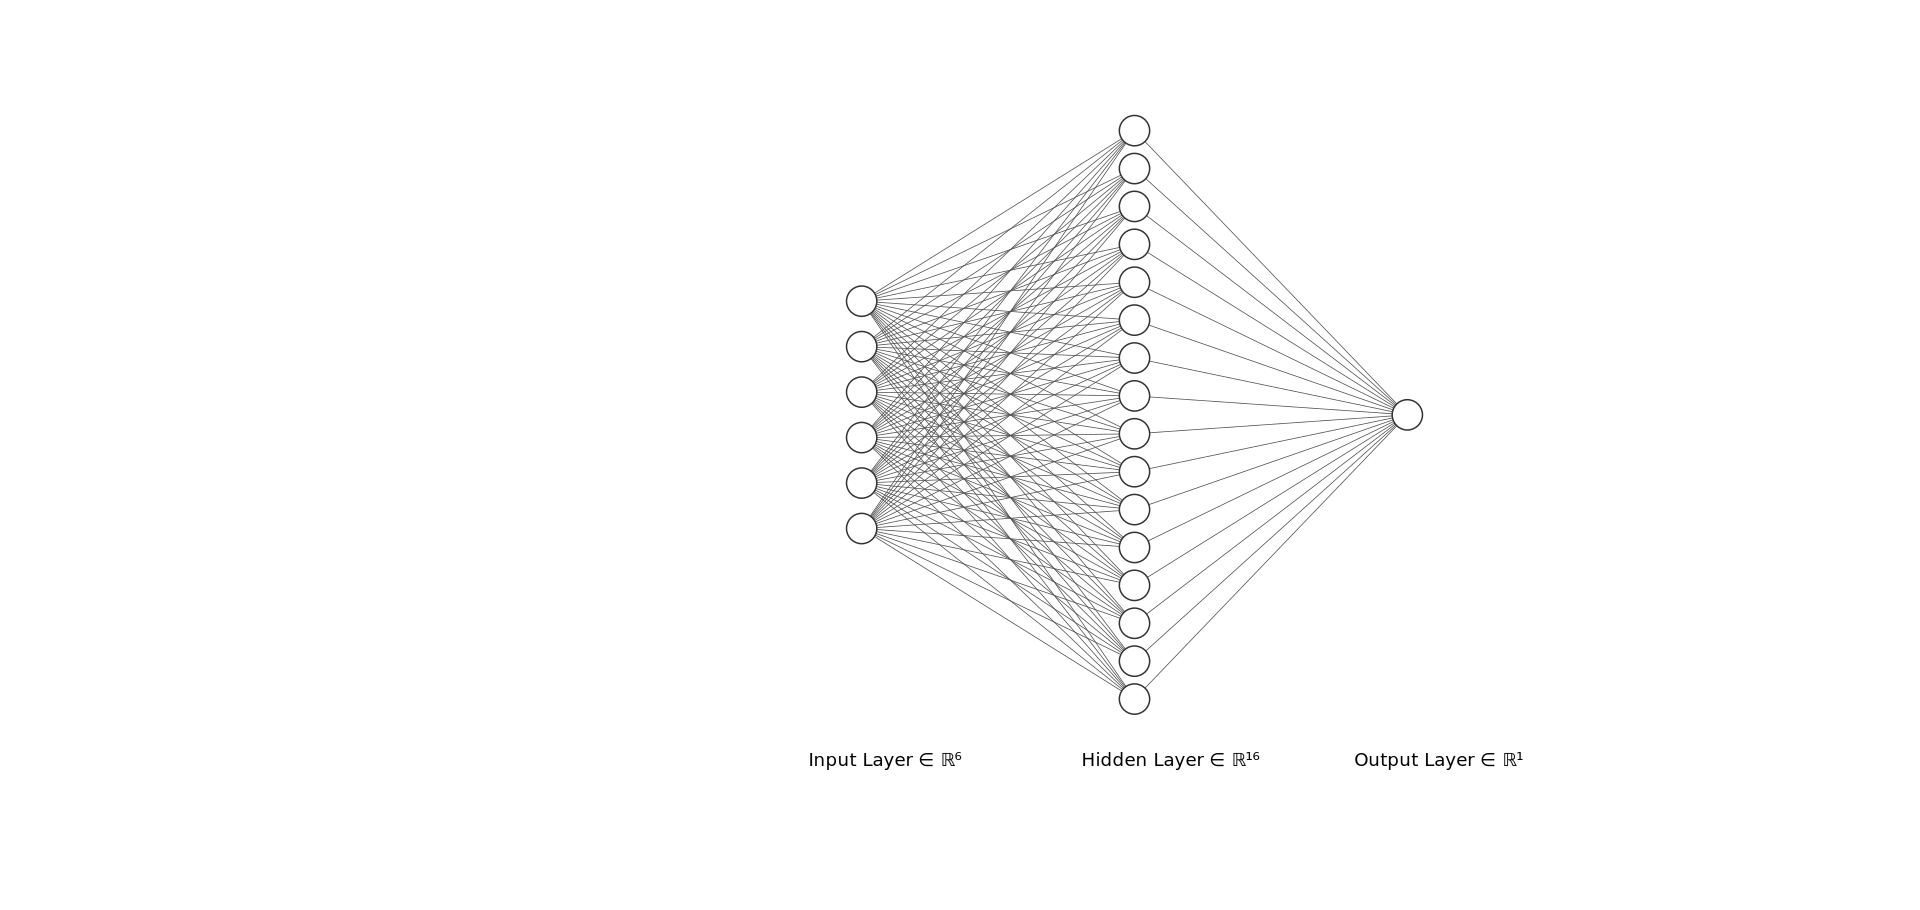
\includegraphics[width=0.8\columnwidth]{images/nn.png}
    \centering
    \caption{A fully-connected neural network with 6 nodes in the input layer, an arbitrary number of nodes in the hidden layer, and a single node in the output layer.}
    \label{fig:NN}
\end{figure}

The inputs to this neural network are the samples from two discrepant datasets with the relevant cosmological parameters, and the output node is a 1D tension coordinate. Due to its popularity and effectiveness in modern deep learning applications \cite{Nwankpa2018}, a rectified linear unit (ReLU) \cite{Nair2010} is chosen as the activation function between the hidden layer and output layer. We can express our neural network as
\begin{equation}
    t = T(\theta; w) = \sum_i w^{(2)}_i \ \textrm{ReLU} \bigg( \sum_j w^{(1)}_{ij} \theta_j + b_i \bigg)
\end{equation}
where we have cosmological parameters $\theta_{j}$, neural network weights $w^{(l)}_{ij}$, and bias $b_i$. As mentioned in Section \ref{non_gaussian}, the loss function is the Bayes Factor calculated in the 1D tension coordinate.

Training this neural network is different from training one for a classification problem. Unlike the 'traditional' method of approximating the gradient using small batches of training data \cite{Keskar2017}, we use all the data points of the two datasets to compute our gradient, and hence calculate the loss function. We do this to provide the Bayes factor, which is our loss function, with a substantial amount of data points to better quantify tension. However, we note that no attempts were made in this paper to experiment with a smaller batch size, e.g. half the data points, thus we cannot confirm that an optimal method was employed here. We use the recently popularised Adam optimisation algorithm \cite{Kingma2017} as our stochastic gradient descent method, with an initial learning rate of $10^{-4}$.


\subsection{Numerical Calculation of Bayes Factor}

The calculation of the marginalised Bayes factor $R_t$ forms part of the neural network's optimisation loop. This requires the speed of the numerical computation of $R_t$ to be as rapid and efficient as possible. More importantly, the gradient-based optimisation method chosen necessitates the calculation of $R_t$ to be smooth and differentiable. This rules out the use of binning methods that rely on square top-hat functions. Thus to numerically calculate $R_t$, we rely on a non-parametric smoothing method known as the \textit{kernel density estimator} \cite{Rosenblatt1956, Silverman1986} to estimate the marginalised posteriors and prior in Equation \ref{margin_R}. This method uses (weighted) samples of distributions to makes these approximations.

For an arbitrary one-dimensional weighted dataset $\{(x_{i}, w_{i}), \, i = 1, \dots , n, \, \sum_i^N w_{i} = 1\}$, the kernel density estimator is expressed as
\begin{equation}
    \hat{f}_h (x) = \frac{1}{h} \sum_{i = 1}^{n} w_{i} K \bigg( \frac{x - x_{i}}{h} \bigg)
\end{equation}
where $K$ is the kernel function and $h$ the bandwidth parameter (a notation first introduced by Rosenblatt \cite{Rosenblatt1956}). The kernel function has to satisfy $\int_{\infty}^{\infty} K(x) \, \textrm{d} x = 1$, thus we pick the kernel to be a Gaussian given by
\begin{equation}
    K(x) = \frac{1}{\sqrt{2\pi h^2}} e^{-x^2}.
\end{equation}
Selecting the bandwidth parameter is more complicated. A review of the various choices of bandwidth parameters and bandwidth selection methods can be found in \cite{Turlach1993}. Given our choice of a Gaussian kernel, we choose the general rule of thumb, also known as Scott's rule, as our bandwidth. This rule is written as $h = n_{\textrm{eff}}^{d + 4}$, where $n_{\textrm{eff}} = (\sum w_{i})^2 / {\sum {w_{i}}^2}$ is the effective number of data points and $d$ is the number of dimensions of the distribution being estimated. This setup allows us to effectively approximate unimodal distributions, which the majority of cosmological datasets are.

We use this kernel density estimator to provide an estimate of the marginalised posteriors and the prior found in Equation \ref{margin_R}, which can be denoted by $\hat{\mathcal{P}}_A^{t}$, $\hat{\mathcal{P}}_B^{t}$ and $\hat{\pi}^{t}$ respectively. This gives a marginalised Bayes Factor of
\begin{equation}
    R_t \approx \sum_{j = 1}^{M} \frac{\hat{\mathcal{P}}_A^{t}(t_j) \hat{\mathcal{P}}_B^{t}(t_j)}{\hat{\pi}^{t}(t_j)} \Delta t,
\end{equation}
where we sample the posteriors and prior at points $t_j$ in the 1D tension coordinate at regular intervals, separated by width $\Delta t$.

In practice, we find it more effective to use $\log R_t$ instead of $R_t$ as our loss function for the neural network. If we were to use $R_t$, the optimisation steps taken by the neural network becomes increasing small and inconsequential as $R_t \to 0$. On the other hand, $\log R_t$ with its range of $(-\infty, \infty)$ allows gradient descent to make bolder steps towards the local minimum. Taking the natural log of the Bayes factor also prevents underflow issues for extremely discrepant datasets ($R_t \to 0$) by exploiting the LogSumExp method to calculate the posteriors, prior and ultimately $\log R_t$. The LogSumExp method of calculating a log probability can be found in the source code of \texttt{Scipy}'s \texttt{gaussian\_kde} method \cite{Scipy2020}.

An alternative method to calculating $R_t$ that might be viable is using a histogram density estimator with a Gaussian envelope rather than a top-hat function \cite{Schutt2017}. However, we find that this method suffers from underflow problems, which undesirably results in $\log R_t \to - \infty$. Hence, we stuck with the Gaussian kernel density estimator.



% Let us begin by defining a typical histogram as a probability density estimator. For an arbitrary weighted dataset $\{(X^{(i)}, w^{(i)}), \, i = 1, \dots , N, \, \sum_i^N w^{(i)} = 1\}$ of range $[x_0, x_1]$, we form histogram bins $b^{(j)}$ with constant bin width $\Delta$ and a centre $c^{(j)}$. The interval of $b^{(j)}$ is defined as $[x_0 + j\Delta, x_0 + (j+1)\Delta]$. The probability estimate of values in the $j$th bin is then given by
% \begin{equation} \label{tophat}
%     \hat{p}^{(j)}(x) = \frac{1}{\Delta} \sum_{i=1}^{N} w^{(i)} F(X^{(i)} - c^{(j)})
% \end{equation}
% where $x \in b^{(j)}$, and  $F$ is a top-hat function of width $\Delta$ centred at zero.

% With this definition of a histogram, the marginalised Bayes factor $R_t$ can be approximated as
% \begin{equation}
%     R_t \approx \sum_{i}^{N_\pi} \frac{\Big(\sum_{c_A^{(j)} \in b_\pi^{(i)}} \Delta_A \hat{p}_A^{(j)}\Big) \Big(\sum_{c_B^{(j)} \in b_\pi^{(i)}} \Delta_B \hat{p}_B^{(j)}\Big)}{\Delta_\pi \hat{p}_\pi^{(i)}},
% \end{equation}
% where we have two datasets $A$ and $B$ with a shared prior $\pi$.

% However, we have a big problem. The optimisation of the neural network uses a gradient-based method, which requires our computation of $R_t$ to be smooth and differentiable everywhere. The top-hat function $F$ in Equation \ref{tophat} is not smooth. Fortunately, we can replace $F$ with a smooth function with non-extreme derivatives to approximate a histogram. We choose a Gaussian to be the replacement of $F$ \cite{Schutt2017}, such that
% \begin{equation}
%     F(x) = \frac{1}{\sqrt{2\pi \sigma^2}} \exp \bigg( {-\frac{x^2}{2 \sigma^2}} \bigg)
% \end{equation}
% with $\sigma = \Delta / 2$. We find using such a Gaussian envelope is able to approximate a top-hat histogram quite well. [Give chi-squared?]

% In practice, we find it more effective to use $\log R_t$ instead of $R_t$ as our loss function for the neural network. If we were to use $R_t$, the optimisation steps taken by the neural network becomes increasing small and ineffective as $R_t \to 0$. On the other hand, $\log R_t$ with its range of $(-\infty, \infty)$ allows gradient descent to make more confident steps towards the local minimum.

% Note that instead of using a histogram as a probability density estimator, an alternative method is to use a Gaussian kernel density estimator (KDE) \cite{Silverman1986}. However, we find that the histogram method provides more stability and computational efficiency during gradient descent, hence the decision to stick with histograms with a Gaussian envelope function.



% https://stats.stackexchange.com/questions/143284/density-estimation-and-histograms

\subsection{Toy Examples}

\begin{figure*}
    \includegraphics[width=0.9\textwidth]{../plots/toy_wide.png}
    \centering
    \caption{The main contour plots illustrate the iso-tension coordinate hypersurfaces shaped by the neural network after training for 500 epochs on our toy examples. a) shows two Gaussian distributions and b) shows a Gaussian distribution accompanied by a 'banana-shaped' distribution. The faded blue distribution in the background is the prior. The smaller plots along the $x$ and $y$ axes show the marginalised distributions of these toy examples in their respective axes.}
    \label{fig:toy}
\end{figure*}

Algorithm \ref{algo} takes us through the training of our neural network using \texttt{PyTorch}-esque language. Note that the learning rate of the optimisation method and number of epochs can be adjusted in order to reach a stable local minimum of the Bayes Factor $R_t$.
\begin{algorithm}[H]
\caption{Training of Neural Network}\label{algo}
    \begin{algorithmic}[1]
    % \Procedure{Euclid}{$a,b$}\Comment{The g.c.d. of a and b}
    \State $X_A \gets $ Dataset A; $w_A \gets $ Weights A 
    \State $X_B \gets $ Dataset B; $w_B \gets $ Weights B
    \State $X_\pi \gets $ Prior; $w_\pi \gets $ Prior Weights
    \State
    \State $net \gets $ NeuralNetwork(in=6, hidden=4096, out=1)
    \State $optim \gets $ AdamOptimizer($net.parameters()$, learning\_rate=$10^{-4}$)
    \State $loss \gets $ LogBayesFactor()
    \State $epochs \gets 1000$
    \State
    \For{$i \gets 0$ to $epochs$}
        \State $X_A^t \gets net(X_A)$ \Comment{Tension coordinates}
        \State $X_B^t \gets net(X_B)$
        \State $X_\pi^t \gets net(X_\pi)$
        \State
        \State $R_t \gets loss(X_A^t, X_B^t, X_\pi^t, w_A, w_B, w_p)$
        \State $R_t.backward()$ \Comment{Compute gradients of neural network parameters}
        \State $optim.step()$ \Comment{Make gradient descent step}
    \EndFor
    \State
    \State \textbf{return} $net$
    \end{algorithmic}
\end{algorithm}

Before applying the neural network onto cosmological datasets, we first verify our method using toy datasets. We generate 10000 samples from each of the distributions described below to create our toy datasets.

The very simplest case to begin with would be two discrepant 2D Gaussian distributions, that are also discrepant in each dimension individually. In our example, we place these two distributions around $5\sigma$ apart, and encase them in a square prior, as seen in Figure \ref{fig:toy}(a).  Our neural network is able to fit rough hyperplanes perpendicular to a line connecting the two distributions. This is a result that agrees with the analytical tension coordinate for the Gaussian case derived in Section \ref{gaussian_tension}.

The next example can be seen in Figure \ref{fig:toy}(b). We are still working in two dimensions, but now we have a Gaussian distribution accompanied by a concave quarter-circle distribution. These two distributions are discrepant in two dimensions, but have a considerable overlap in their 1D marginalised distributions. We use this example, albeit an exaggerated example, to reinforce the idea that multi-dimensionality is able to hide non-linear tensions. With this setup, we expect the hypersurfaces, or more simply the contour lines, to be shaped around the 'banana-like' distribution, with directions of maximum tension radiating outwards from the central Gaussian distribution. This is exactly what we see from our results, as illustrated in Figure \ref{fig:toy}(b).

It is crucially important to note that the statistical power of our neural network only lies in the region between our two distributions, and begins to falter as we navigate further away. This effect is obvious in both of our toy examples. In the first case, we see the contour lines bending in the bottom-right and upper-left corners of the plot. In the second example, the curve of the contours do not exactly follow the outer curve of the 'banana-shaped' distribution as we would have expected if the neural network was able to extrapolate well.


\subsection{Cosmological Dataset}

In this paper, we work solely with the cosmological datasets collected by the DES and the \textit{Planck} satellite. We choose these two datasets because of the well reported tensions between them in recent years \cite{Handley2019, Lemos2020}. The tensions mentioned in Section \ref{intro} of this paper, such as the $3\sigma$ tension in the $\Omega_m$ and $\sigma_8$ plane, also exist between these two datasets.

We use the following six cosmological parameters -- baryon density $\Omega_b h^2$, matter density parameter $\Omega_m$, Hubble constant $H_0$, optical depth to reionisation $\tau$, matter fluctuation amplitude $\sigma_8$, and scalar spectral index $n_s$. The derived parameters of $\Omega_m$, $H_0$ and $\sigma_8$ are chosen over the three other independent cosmological parameters of dark matter density $\Omega_c h^2$, angular acoustic scale $100 \theta_*$ and log of primordial fluctuation amplitude $\log A_s$,  because tensions in these parameters are well-known. Applying our neural network to these parameters with established discrepancies allows us to verify and reinforce the existing tension in them.

We obtain the DES Y1 and \textit{Planck} datasets from \cite{Dataset}, and use the prior from the DES dataset as the prior for calculating the Bayes factor. This source provides nested sampling chains for all of the relevant independent, derived and nuisance parameters of both datasets. We use the \texttt{anesthetic} \texttt{Python} library \cite{anesthetic} to extract weighted samples from the nested sampling chains. 


\subsection{Identifying the Source(s) of Tension} \label{section:source}

We first train our neural network on all six cosmological parameters to produce a 1D tension coordinate. This gives us an initial intuition of the maximum tension that can be formed between the DES Y1 and \textit{Planck} datasets. To evaluate the contribution of each parameter to the tension, we replace a single parameter with noise and feed this into the trained neural network, effectively eliminating its influence on the tension. We accomplish this by randomly permuting the values of the single parameter across all samples, while maintaining the order of the other parameters. By removing the effects of a more influential parameter, we would expect the two datasets to be in much less tension when compared to removing a less significant parameter.

To verify our results from training our neural network on all six parameters, we make pair-wise comparisons between the six parameters. We construct separate neural networks with two input nodes for each of the fifteen combinations of parameter pairs. This allows us to identify pairs of parameters that contribute most to the discrepancy between the two datasets. This hopefully will also allow us to rank the importance of each parameter, and compare the results obtained here against those from the above paragraph.


\section{Results and Discussion}

In this section, instead of expressing the 1D tension coordinate in its 'raw' form, we transform the coordinate to one where the prior is uniform and flat. To perform this transformation, we use the cumulative distribution function of the marginalised prior distribution, which we denote as $\Pi^t(t) = \pi^t(X_\pi^t < t)$, to transform the posteriors and priors such that $\hat{\pi}^{t'}_P = \Pi(X_\pi^t)$, $\hat{\mathcal{P}}_A^{t'} = \Pi(X_A^t)$ and $\mathcal{P}_B^{t'} = \Pi(X_B^t)$. This gives a range of $[0, 1]$ for the transformed 1D tension coordinate $t'$. We will drop the prime from here on, and let $t$ refer to the transformed coordinate. Note that this transformation does not affect the marginalised Bayes Factor $R_t$.

\subsection{Six Parameters} \label{section:six}

We train our neural network for 500 epochs, starting off with a learning rate of $10^{-4}$ for our Adam optimiser and dropping to $10^{-5}$ as we approach $\log R_t \approx -8$. We find that this setup gives a quick and somewhat stable gradient descent. Knowing that neural networks are only able to optimise to a local minimum rather than the global minimum, we perform 10 training repetitions to give a rough estimate of the lowest possible marginalised Bayes factor. 

From the 10 training runs, we obtain a marginalised Bayes factor of $\log R_t = -16.8 \pm 0.5$. If we use the tension coordinate derived from the Gaussian assumption detailed in Section \ref{gaussian_tension}, we get a marginalised Bayes Factor of only $\log R_t = -0.94$. The significant difference between theses two values gives an initial impression of the neural network's ability to identify a tension coordinate that maximises tension. The density plots of the marginalised posteriors drawn in Figure \ref{fig:six_compare} further demonstrates how the neural network is able to significantly amplify the distance and discrepancy between the two datasets.

\begin{figure}
    \includegraphics[width=0.8\columnwidth]{../plots/six_1d_compare.png}
    \centering
    \caption{Density plots of the marginalised posteriors of the DES and Planck datasets, and their prior, in the transformed 1D tension coordinate. (a) uses the Gaussian assumption described in Section \ref{gaussian_tension} and (b) uses the neural network approach. They give marginalised Bayes factors of $\log R_t = -0.94$ and $\log R_t = -16.8 \pm 0.5$ respectively. Note that the prior is uniform across the range of the tension coordinate, and the bend at the edges of the prior is an just artefact of the kernel density estimator method.}
    \label{fig:six_compare}
\end{figure}

The neural network's effectiveness in capturing the non-linearity of the tension between the two datasets is illustrated in Figure \ref{fig:six}. In these 2D plots, we observe how our method is able to carve out hypersurface contours isolating the narrower distribution of the \textit{Planck} dataset. For some of the plots, including the $\Omega_b h^2$ - $\tau$ and $\sigma_8$ - $\tau$ plots, the contours even encircle around the \textit{Planck} dataset. The plots between the tension coordinate and cosmological parameters in the final row of the same figure also begin to describe how each parameter contributes to the tension. However, the wide constraints of the DES dataset renders an analysis via correlation coefficients inconclusive. 

\begin{figure*}
    \includegraphics[width=\textwidth]{../plots/six.png}
    \centering
    \caption{The background of these plots shows the two-dimensional marginalised distributions of the DES and \textit{Planck} datasets, and the prior. These distributions are represented by solid iso-probability contours containing $68\%$ and $95\%$ of the marginalised probability mass. The foreground in these plots, bar the last row, illustrates contour plots of the iso-tension coordinate hypersurfaces. These contour plots are drawn by varying the two relevant cosmological parameters and fixing the other four, then feeding these data points into the trained neural network. The four data points are fixed at the weighted parameter means of the combined DES-\textit{Planck} dataset. The final row plots the tension coordinate $t$ against the six cosmological parameters, visually emphasising the maximum possible tension found between these two datasets. The marginalised Bayes factor for this particular optimised neural network is computed to be $-16.9$, while we get an estimate of $\log R_t = -16.8 \pm 0.5$ from 10 separate gradient descent runs on the same neural network setup.}
    \label{fig:six}
\end{figure*}

Before we go further, it is immensely important to reiterate the fact that many local minima exist in our loss function landscape. The many possibilities of a maximum tension coordinate implies that there are a multitude of forms in which the iso-tension coordinate hypersurfaces can be drawn. Figure \ref{fig:six} is only one example out of the many configurations, thus drawing conclusions from solely this figure is not a particularly good course of action.

To identify the parameters which contribute most to the tension, we introduce noise to a single parameter by randomly shuffling the values of the parameter across all samples of the dataset, while leaving the order of the other parameters undisturbed. This 'new' dataset is then fed into the trained neural network from before, and a marginalised Bayes factor is calculated from the output. We do this for each of the six parameters. The outcome from this procedure is detailed in Table \ref{table:shuffled}.

\begin{table}
\begin{ruledtabular}
\begin{tabular}{lr}
    Shuffled Parameter & $\log R_t$ \\
    \colrule
    $H_0$           & $-1.9 \pm 0.3$ \\
    $\Omega_b h^2$  & $-2.0 \pm 0.3$ \\
    $\Omega_m$      & $-2.6 \pm 0.3$ \\
    $n_s$           & $-3.1 \pm 0.4$ \\
    $\sigma_8$      & $-6.4 \pm 0.8$ \\
    $\tau$          & $-7.3 \pm 0.9$ \\
    \colrule
    None            & $-16.8 \pm 0.5$ \\
\end{tabular}
\end{ruledtabular}
\caption{Marginalised Bayes factors from using a dataset containing a single shuffled parameter as input to a trained neural network with six input nodes, as detailed in Section \ref{section:six}. The more positive the $\log R_t$, the more influential the parameter is to defining the tension coordinate.}
\label{table:shuffled}
\end{table}

A more positive $\log R_t$ (less tension) here indicates a more important parameter in defining the tension coordinate, since shuffling its values effectively removes the influence of the parameter. One can think of the absolute difference between the unadulterated dataset and the shuffled dataset to be a value quantifying the contribution to the tension of a particular parameter. The larger the difference, the larger the contribution. 

The result here points to $H_0$ and $\Omega_b h^2$ being the largest contributor to the tension, with $\Omega_m$ coming in at a close third. This result supports the examples of cosmological tensions mentioned in Section \ref{intro}, particularly for $H_0$ and $\Omega_m$. The result also indicates that $\tau$ and $\sigma_8$ are the least significant influencers of the tension. It is not unexpected for the former since the DES dataset doesn't constrain $\tau$. However, it is curious that the latter is considered to be of low significance given the existence of the $\Omega_m$ - $\sigma_8$ tension in the community. Finally, we notice a considerable contribution to tension from the $n_s$ parameter. This is somewhat unanticipated as DES does not set any constraints on $n_s$. A density plot from the perspective of the $n_s$ parameter (can be inferred from the bottom-right plot in Figure \ref{fig:six}) also does not reveal any obvious tensions. The neural network appears to have picked out a non-trivial source of tension, but further exploration is needed to better understand this behaviour.


\subsection{Pair-wise Comparison} \label{section:pair}

We train our neural network for 500 epochs with parameter pairs as the input, and maintain a learning rate of $10^{-4}$ with the Adam optimiser. We perform 5 training repetitions for each parameter pair. The results are given in Table \ref{table:pairwise}. It is important to note here that there is a nuanced distinction between the results of this section and the previous section. Here, we seek for parameters \textit{containing} the most tension via parameter pairs, whilst in the previous section we attempted to identify parameters which \textit{contributed} most to the tension in the six-dimensional parameter space.

\begin{table}
\begin{ruledtabular}
\begin{tabular}{l r r}
    Parameter Pair & $\log R_t$ & Rank \\
    \colrule
    $\Omega_b h^2$ - $\Omega_m$ &	$-3.66 \pm 0.16$ & $1$  \\
    $\Omega_b h^2$ - $H_0$      &	$-3.26 \pm 0.11$ & $4$  \\
    $\Omega_b h^2$ - $\tau$     &	$-2.17 \pm 0.44$ & $10$ \\
    $\Omega_b h^2$ - $\sigma_8$ &	$-3.40 \pm 0.17$ & $3$  \\
    $\Omega_b h^2$ - $n_s$      &	$-1.95 \pm 0.22$ & $12$ \\
    $\Omega_m$ - $H_0$          &	$-3.02 \pm 0.21$ & $7$  \\
    $\Omega_m$ - $\tau$         &	$-3.23 \pm 0.22$ & $6$  \\
    $\Omega_m$ - $\sigma_8$     &	$-2.73 \pm 0.25$ & $8$  \\
    $\Omega_m$ - $n_s$          &	$-2.62 \pm 0.41$ & $9$  \\
    $H_0$ - $\tau$              &	$-3.57 \pm 0.04$ & $2$  \\
    $H_0$ - $\sigma_8$          &	$-3.25 \pm 0.06$ & $5$  \\
    $H_0$ - $n_s$               &	$-1.94 \pm 0.47$ & $13$ \\
    $\tau$ - $\sigma_8$         &	$-2.13 \pm 0.17$ & $11$ \\
    $\tau$ - $n_s$              &	$-0.73 \pm 0.01$ & $15$ \\
    $\sigma_8$ - $n_s$          &	$-1.86 \pm 0.06$ & $14$ \\
    \hline \hline
    Parameter & Mean $\log R_t$ & Rank \\
    \colrule
    $\Omega_m$      & $-3.05 \pm 0.25$ & 1 \\
    $H_0$           & $-3.01 \pm 0.18$ & 2 \\
    $\Omega_b h^2$  & $-2.89 \pm 0.22$ & 3 \\
    $\sigma_8$      & $-2.68 \pm 0.14$ & 4 \\
    $\tau$          & $-2.37 \pm 0.17$ & 5 \\
    $n_s$           & $-1.82 \pm 0.24$ & 6 \\
\end{tabular}
\end{ruledtabular}
    
\caption{The upper table details the marginalised Bayes factors calculated from trained neural networks with parameter pairs as its input. We rank the pairings by increasing $\log R_t$, or decreasing tension, in the rightmost column. The lower table gives the mean $\log R_t$ from the results of parameter pairings containing the respective parameter.}
\label{table:pairwise}
\end{table}

The results here generally correlate well with the results from the previous section. We still find that $\Omega_m$, $H_0$ and $\Omega_b h^2$ are the top three parameters containing the most tension, albeit permuted in a slightly different order. The largest differences compared to the previous section's results is the increase of tension found in $\sigma_8$ and the drop in rank to last for $n_s$.

The rank of parameters containing the most tension here is more in line with what we would expect. The unconstrained parameters of the DES dataset -- $\tau$ and $n_s$, are now considered as the least discrepant. On the opposite end of the scale, the results are able to reinforce known cosmological tensions found in $H_0$ and the $\Omega_m$ - $\sigma_8$ plane. However, it is interesting to note that our neural networks do not consider the pairing of $\Omega_m$ - $\sigma_8$ to contain the most tension, but find pairings such as $\Omega_b h^2$ - $\Omega_m$ and $H_0$ - $\tau$ to have the largest discrepancies. A possible reason for these large tensions could be the significant difference between the widths of the \textit{Planck} and DES datasets for these parameters. For example, one could argue that the wide constraint favouring a larger value of $H_0$ or $\Omega_b h^2$ (or disfavouring a lower value) is a key contributor to the tension. 

It is important to highlight that despite $n_s$ ranking as the parameter containing the least tension, a mean marginalised Bayes factor of $\log R_t = -1.82 \pm 0.24$ is by no means an indication of a concordant parameter. This value of $R_t = 0.162$ is definitely considered to be in tension, but care needs to be taken here. Is the source of discrepancy from the other parameters paired to $n_s$, or does $n_s$ itself contain some tension? These results do not reveal such information, and more work needs to be done to isolate each individual parameter.


\section{Conclusions}

Applying our neural network to the six cosmological parameters of $\Omega_b h^2$, $\Omega_m$, $H_0$, $\tau$, and $\sigma_8$ and $n_s$ yields a maxmimum tension of $\log R_t = -16.8 \pm 0.5$ between the \textit{Planck} and DES datasets. The neural network was successful in capturing the non-linearity of the iso-tension coordinate hypersurfaces, and exaggerating the distance between the two datasets. The marginalised Bayes factor in this tension coordinate is significantly more discrepant than if we were to use an analytical approach assuming that the distributions were Gaussian.

We used two different methods in an attempt to identify the source of and contribution to tension from each parameter. We found that $H_0$, $\Omega_m$ and $\Omega_b h^2$ were the three main contributors to tension in both methods. This lends support to the well-established tensions found in $H_0$ and the $\Omega_m$ - $\sigma_8$ plane. On the lower end of the scale of lesser tension, there were some disagreements between the two approaches. The first approach ranked the unconstrained parameter in the DES dataset of $n_s$ to be more influential than one would expect, and $\sigma_8$ to be less important. The second approach gave results that were more in line with what was expected, where the unconstrained parameters in the DES dataset of $n_s$ and $\tau$ were ranked as the least discrepant.

We mentioned in Section \ref{intro} that tensions could be an artefact of systematic errors, or could point to new physics. These results unfortunately do not hint at either direction, however it reinforces on the direction in which current research is heading toward. This paper points to $H_0$, $\Omega_m$ and $\Omega_b h^2$ as highly discrepant cosmological parameters, hence these are worthwhile areas to be looking into. It would also be interesting to see this method applied to other dataset pairings, which could potentially reveal new underlying cosmological tensions.



\begin{acknowledgments}

\end{acknowledgments}

\appendix

\section{Appendixes}

\section{A little more on appendixes}


\subsection{\label{app:subsec}A subsection in an appendix}




% The \nocite command causes all entries in a bibliography to be printed out
% whether or not they are actually referenced in the text. This is appropriate
% for the sample file to show the different styles of references, but authors
% most likely will not want to use it.

\bibliography{apssamp}% Produces the bibliography via BibTeX.

\end{document}
%
% ****** End of file apssamp.tex ******